\section{Patient-Level Clustering Extension: Results}\label{sec:extension_results}

The new analyses identify repeatable groupings of cognitive scores, while leaving their interpretation as discrete clinical phenotypes unresolved. Results below use the earliest eligible assessment from each of 7{,}285 patients, with 5{,}828 discovery and 1{,}457 validation patients. They are not direct performance comparisons with the historical assessment-level UMAP analysis because the cohort, representation and validation design differ.

\subsection{Original-Space Comparisons and Cluster Count}

Table~\ref{tab:extension_benchmarks} reports representative solutions selected using discovery data. Two-group k-means and PAM were favored in the reference six-domain representation. Direct HDBSCAN assigned all observations to noise under both tested minimum cluster sizes, whereas UMAP+HDBSCAN recovered groups. Increasing UMAP neighborhood size from 15 to 50 changed the recovered count and reduced measured-domain separation. This supports checking embedding-derived partitions in the measured features; it does not rule out other density-model settings.

\begin{table}[htbp]
\centering\small
\caption{Selected patient-level models. Silhouettes are calculated in each row's stated representation; different geometries are not directly comparable. All listed solutions have 100\% validation coverage.}
\label{tab:extension_benchmarks}
\begin{tabular}{p{0.31\textwidth}p{0.22\textwidth}rrr}
\toprule
Model & Representation & $k$ & Discovery & Validation \\
\midrule
K-means & Robust domains & 2 & 0.666 & 0.649 \\
Sampled PAM & Robust domains & 2 & 0.553 & 0.540 \\
Full Gaussian mixture & Robust domains & 8 & 0.117 & 0.118 \\
Tied Gaussian mixture & Robust domains & 5 & 0.548 & 0.535 \\
K-means & PC1 residuals & 3 & 0.547 & 0.532 \\
K-means & 14 tests & 2 & 0.406 & 0.399 \\
UMAP+HDBSCAN & Robust domains & 2 & 0.389 & 0.400 \\
\bottomrule
\end{tabular}
\end{table}

The k-means discovery-silhouette search selected two groups in all 20 stochastic imputations. This is a consistent choice among $k=2,\ldots,8$, not a test against one population. The eight-component full Gaussian domain model also reaches the search limit. Accordingly, neither silhouette selection nor a boundary BIC minimum identifies a unique natural cluster count.

\subsection{Independent Imputation and Patient Stability}

Two- and three-group k-means were highly repeatable conditional on the robust-domain representation and bounded Bayesian imputation model (Table~\ref{tab:extension_stability}). Fixed three-group patient subsampling gave mean pairwise validation ARI 0.968, and varying clustering seeds with the input fixed gave ARI 1.000. Mean matched Jaccard values for the three groups were 0.994, 0.959 and 0.947. These measures describe repeatability within the specified pipeline, not evidence that its groups correspond to distinct clinical entities.

\begin{table}[htbp]
\centering\small
\caption{Pairwise agreement on the same validation patients after independent fits across 20 stochastic imputations. Percentiles describe dependent pairwise comparisons and are not confidence intervals.}
\label{tab:extension_stability}
\begin{tabular}{lrrr}
\toprule
Method & $k$ & Mean ARI & 5th--95th percentiles \\
\midrule
K-means & 2 & 0.959 & 0.944--0.974 \\
K-means & 3 & 0.935 & 0.917--0.951 \\
K-means & 4 & 0.738 & 0.627--0.823 \\
Sampled PAM & 2 & 0.909 & 0.851--0.959 \\
Sampled PAM & 3 & 0.504 & 0.281--0.878 \\
Sampled PAM & 4 & 0.462 & 0.308--0.662 \\
\bottomrule
\end{tabular}
\end{table}

Average-linkage and greedy mean-NMI consensus gave similar agreement for k-means at $k=2$ and $k=3$. Generic NMF aggregation was less reliable: for the two-group k-means ensemble, it reached its iteration limit and collapsed to one assigned group; the requested three-group version produced only two assigned groups. This result concerns ensemble aggregation, not the historical NMF imputation method, and cannot be generalized to all NMF implementations.

\subsection{Scaling, Missingness and Preprocessing Sensitivity}

Robust scaling produced discovery variances of 7.93 for language and 5.76 for orientation, compared with 0.44 for memory. The first component explained 63.3\% of robust-domain variance but loaded predominantly on language and orientation. Narrow central ranges of ceiling-heavy scores amplify their tails under interquartile-range scaling. Equal-domain variance scaling reduced PC1's share to 58.5\% and changed the three-group validation assignments substantially: ARI between the two partitions was only 0.243.

The robust three-group labels had silhouette 0.608 in robust space and 0.440 in equal-domain space. The equal-domain labels had corresponding values 0.172 and 0.283. Figure~\ref{fig:extension_scaling} separates the partition effect from the measurement geometry. Neither geometry is established as clinically correct. Under equal-domain scaling, mean imputation agreement also decreased to 0.769 for two-group k-means and 0.747 for three-group k-means.

\begin{figure}[htbp]
\centering
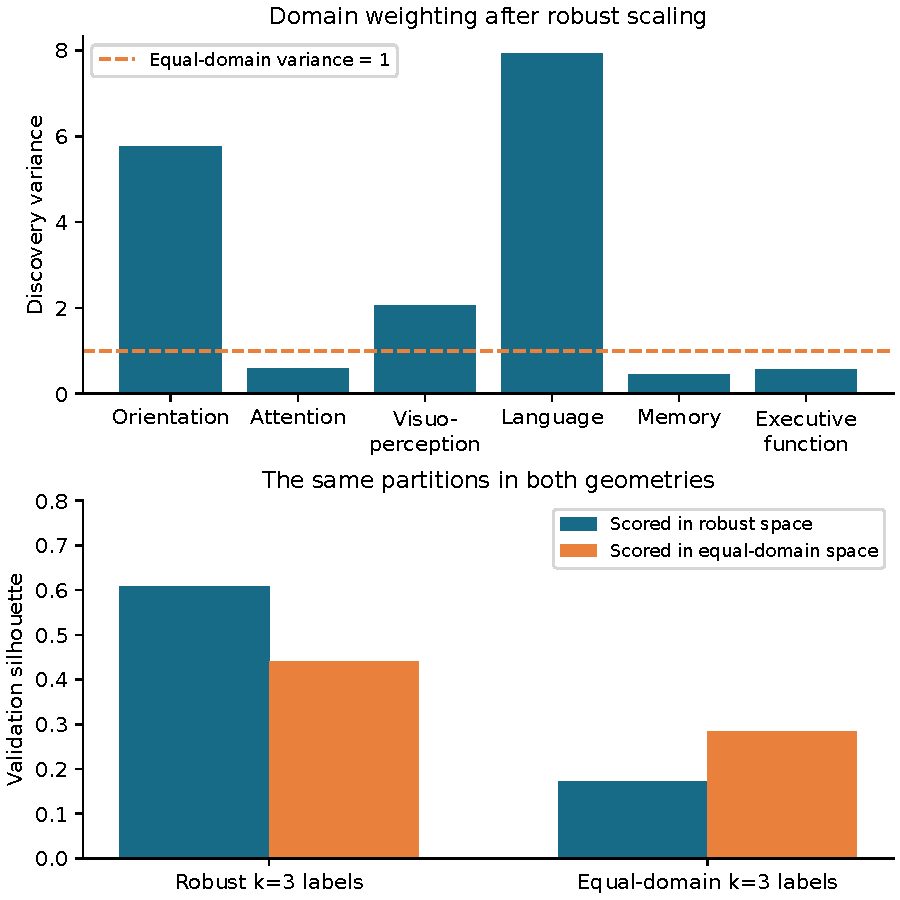
\includegraphics[width=\textwidth]{Figures/extension_scaling_thesis.pdf}
\caption{Scaling sensitivity. Top: domain variances after robust scaling, with unit-variance scaling as a reference. Bottom: the same two three-group partitions evaluated in both geometries. A high silhouette conditional on one geometry does not establish representation-independent subgroups.}
\label{fig:extension_scaling}
\end{figure}

\begin{figure}[htbp]
\centering
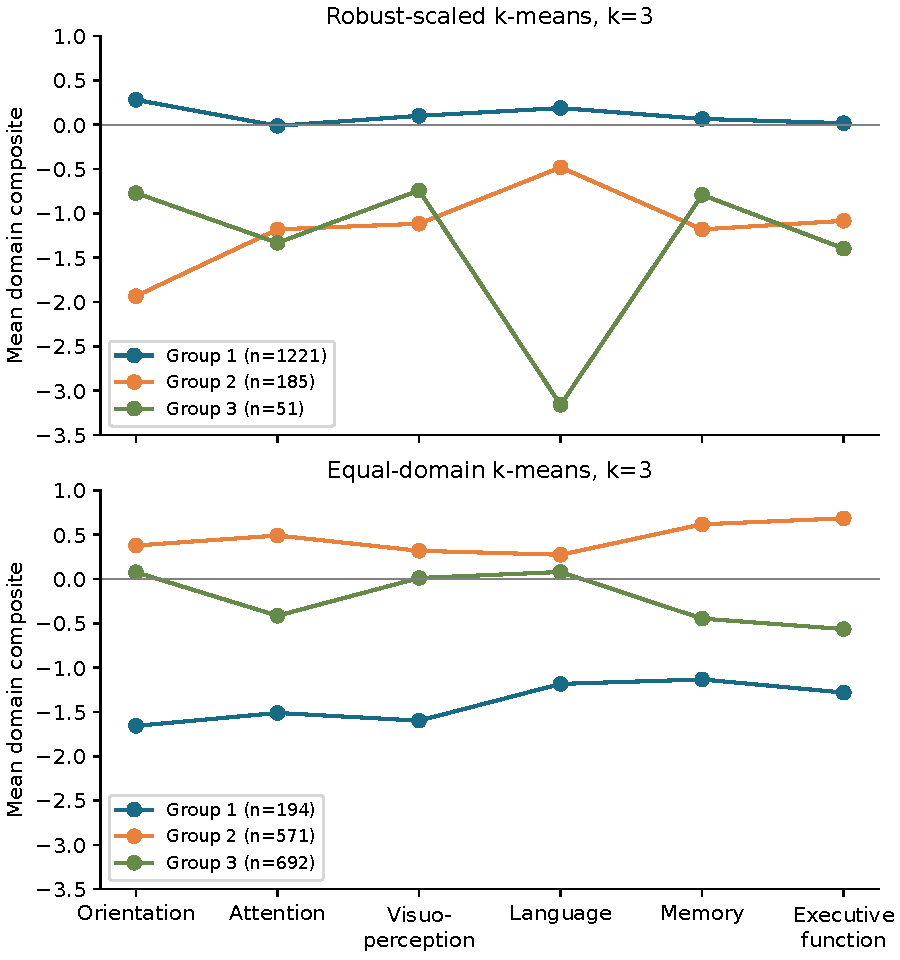
\includegraphics[width=\textwidth]{Figures/extension_profiles_thesis.pdf}
\caption{Validation profiles for fixed three-group k-means under robust and equal-domain scaling. Both panels show the same underlying direction-aligned domain composites. Group numbers and colors are local to each model; matching numbers across panels do not identify the same patients.}
\label{fig:extension_profiles}
\end{figure}

\clearpage
The robust solution contains validation groups of 1{,}221, 185 and 51 patients. Its smallest group shows a pronounced language deficit, whereas equal-domain scaling yields groups of 194, 571 and 692 patients with different profile contrasts (Figure~\ref{fig:extension_profiles}). These exploratory profiles therefore do not justify transferring the historical clinical tier names to the new labels.

Test availability is also associated with the fixed three-group assignments. Cram\'er's $V$ between cluster and missingness was 0.412 for \texttt{MRAVLT075} and 0.371 for \texttt{FEPMR}. Across groups, missingness ranged from 10.2\% to 80.4\% for \texttt{MRAVLT075}, and from 16.1\% to 86.3\% for \texttt{FEPMR}. These descriptive associations do not show that missingness causes the partition, but they prevent interpreting repeatability under one imputation model as freedom from administration effects.

At fixed $k=3$, mean imputation gave ARI 0.921 against the reference assignments, while KNN gave 0.538. Restricting to at least seven observed tests retained 5{,}263 discovery and 1{,}339 validation patients and gave ARI 0.903 on the shared validation subset. Removing clipping gave ARI 0.958. Extending deterministic imputation to 50 iterations converged after 37 and left labels unchanged (ARI 1.000). Independent clustering of validation patients under the frozen discovery transformation gave ARI 0.895; this is an agreement diagnostic rather than another held-out prediction score.

Comparing raw-test aggregation with direction-aligned, standardized domain construction gave three-group ARI 0.703 over all assessments and 0.629 over complete cases. Attention composites correlated $-0.749$ across constructions, highlighting the effect of direction and scale alignment. These descriptive sensitivity checks hold completed values fixed and do not constitute a repetition of the earlier supplementary multiple-imputation and complete-case analyses.

\subsection{Incomplete-Data Mixtures and Continuous References}

Of 32 incomplete-data mixture fits, 28 met the numerical convergence criterion. Table~\ref{tab:extension_mixtures} shows the best BIC fit within each family after the minimum-size and convergence rules. The $t$ family with four degrees of freedom gave the best BIC and validation likelihood among these selected fits. Both $t$ families selected eight components, leaving the optimum unresolved at the upper search limit. Their six-domain silhouettes were low. ICL also selected eight components for both $t$ families, but selected six rather than seven for the contaminated Gaussian.

\begin{table}[htbp]
\centering\small
\caption{Selected observed-data mixtures fitted to 14 incomplete tests. Log likelihood is the mean per validation patient. Silhouette evaluates their assignments in the completed robust six-domain space.}
\label{tab:extension_mixtures}
\begin{tabular}{lrrrr}
\toprule
Family & $k$ & BIC & Validation log likelihood & Silhouette \\
\midrule
Gaussian & 6 & 73{,}878.4 & $-6.076$ & 0.188 \\
Contaminated Gaussian & 7 & 74{,}641.8 & $-6.030$ & 0.154 \\
$t$, df $=10$ & 8 & 69{,}815.8 & $-5.550$ & 0.111 \\
$t$, df $=4$ & 8 & 67{,}545.6 & $-5.341$ & 0.095 \\
\bottomrule
\end{tabular}
\end{table}

These models improve distributional fit without identifying eight validated clinical phenotypes. Multiple components can approximate discrete score masses, skewness and tails. Posterior probabilities quantify membership uncertainty conditional on the selected family and component count, without incorporating uncertainty about model choice or the missingness mechanism.

In the 1{,}000-patient continuous-reference screen, the observed maximum k-means silhouette was 0.676. Its fitted-reference tail fraction was 0.0099, whereas the PC1 dip-statistic tail fraction was 0.9901. The separated positive control recovered two groups with silhouette 0.917. The diagnostics therefore provide different evidence: the silhouette exceeds this particular copula reference, while the projection statistic does not show excess multimodality relative to it. These are descriptive reference comparisons, not an omnibus test establishing clinical phenotypes or excluding all continuous explanations.

\subsection{Longitudinal Findings and Overall Interpretation}

Trajectory eligibility retained 2{,}013 patients: 1{,}590 discovery and 423 validation. All four fitted class counts converged. BIC and validation likelihood improved as classes were added, but every multi-class solution introduced a group below the 5\% expected-membership threshold (Table~\ref{tab:extension_trajectories}). The supplied selection rule therefore retained one trajectory class with continuous patient random effects. Multi-class resampling was not triggered. This is not evidence that all patients recover identically; nonlinear continuous change and small genuine subgroups remain unresolved.

\begin{table}[htbp]
\centering\small
\caption{Patient trajectory models. The 5\% minimum expected discovery-class size is an analysis rule, not a validated clinical threshold.}
\label{tab:extension_trajectories}
\begin{tabular}{rrrr}
\toprule
Classes & BIC & Validation log likelihood & Smallest expected class \\
\midrule
1 & 8{,}376.3 & $-2.598$ & 100.0\% \\
2 & 7{,}572.2 & $-2.403$ & 3.9\% \\
3 & 6{,}806.0 & $-2.290$ & 2.7\% \\
4 & 6{,}465.5 & $-2.212$ & 1.3\% \\
\bottomrule
\end{tabular}
\end{table}

The extension strengthens the evidence that reproducible partitions can be obtained in these cognitive scores. Its principal caution is that repeatability depends on representation and imputation assumptions. Scaling, missingness and distributional family materially affect assignments or component count. Distinct clinical phenotypes remain unconfirmed, and no independent functional outcome was available to establish their utility.
